% !Mode:: "TeX:UTF-8"
%!TEX program  = xelatex

%\documentclass{cumcmthesis}
\documentclass[withoutpreface,bwprint]{cumcmthesis} %去掉封面与编号页



\usepackage{url}
\graphicspath{{Figures/}}
\title{\LARGE 小锅的机器学习笔记--VAE与DDPM}


\schoolname{苏州大学}


\begin{document}
	\makeatletter %使\section中的内容左对齐
	\renewcommand{\section}{\@startsection{section}{300}{0mm}
		{-\baselineskip}{0.5\baselineskip}{\bf\leftline}}
	\renewcommand{\subsection}{\@startsection{section}{300}{5mm}
		{-\baselineskip}{0.5\baselineskip}{\bf\leftline}}
	\renewcommand{\subsubsection}{\@startsection{section}{300}{8mm}
		{-\baselineskip}{0.5\baselineskip}{\bf\leftline}}
 \maketitle

%目录
%\tableofcontents
%\newpage
	\subsection{\Large VAE:}
	\begin{figure}[htbp]
		\centering
		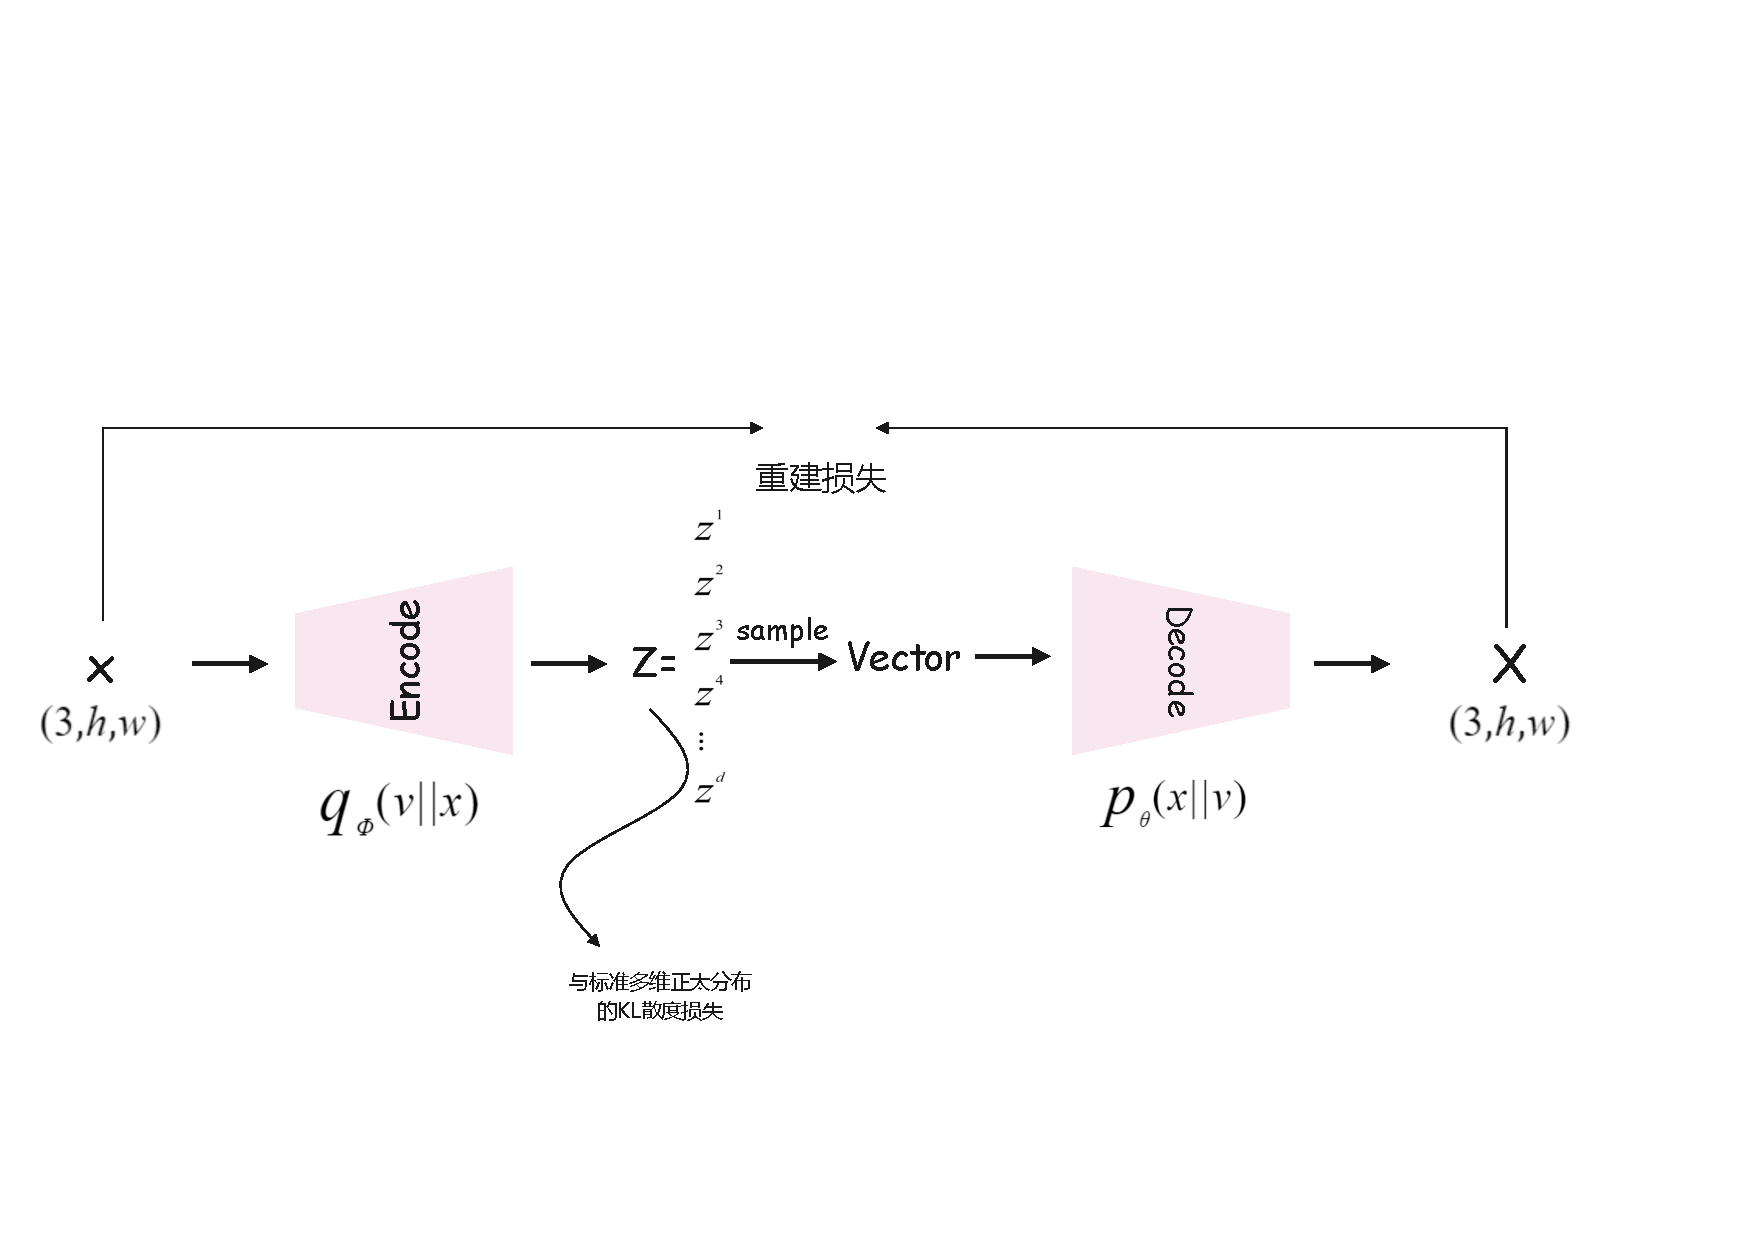
\includegraphics[scale=0.4]{VAE.pdf}
	\end{figure}
	训练的时候,一张图片经过$Encode$编码后,输出向量$Z=\left[z_1,z_2,...,z_d\right]$,其中$z_i=(u_i,\sigma_i)$,我们构建一个$d$维的正太分布:
	$$
		N_{gen}(U,diag(\sigma)) 
	$$
	$$
		\text{其中} \quad \quad U=\left[u_1,u_2,...,u_d\right] \quad \quad \sigma=\left[\sigma_1,\sigma_2,...,\sigma_d \right]
	$$
	从该正太分布中抽样向量$Vector=\left[v_1,v_2,...,v_d\right]$,最后把$Vectot$输出$Decode$中,生成重建图片。
	
	在推理时,丢弃$Encode$,从$d$维度标准正太分布中直接采样出向量$Vector=\left[v_1,v_2,...,v_d\right]$,然后经过$Decode$生成图片。
	
	我们希望$Decode$生成的图片能看,所以有重建损失$L_{restruction}=\Vert image-image_{gen} \Vert^{2}$,由于我们推理的时候是直接从$d$维正太分布中抽样$Vector$的,所以我们希望在训练使构建的分布$N_{gen}(U,diag(\sigma))$尽量的与标准正太分布类似,所以我们有$KL$损失$D_{KL}=KL(N||N_g)$。
	
	下面给出数学推导:
	
	我们记原始数据分布为$p_{data}(x)$, 我们拟合的数据分布为$p_{\theta}(x)$,我们的目标是让拟合的数据分布越来越接近原始分布,也就是我们要最小化$p_{data}(x)$与$p_{\theta}(x)$之间的$KL$散度:
	\begin{align*}
		 &\mathop{min}\limits_{\theta} \left\{\mathbb{E}_{x \sim p_{data}(x)} \left[\log \dfrac{p_{data}(x)}{p_{\theta}(x)} \right] \right\}\\
		 & =  \mathop{max}\limits_{\theta}  \left\{ \mathbb{E}_{x \sim p_{data}(x)} \left[\log {p_{\theta}(x)} \right]  \right\}  \\
		 & \approx \mathop{max}\limits_{\theta} \left\{ \dfrac{1}{|D|}\sum_{x \in D} \left[\log {p_{\theta}(x)} \right] \right\}
	\end{align*}

	其中$D$为数据集,我们用数据集的均值近似期望,其实就是在最大化$p_{\theta}(x)$的似然。
	
	我们引入隐变量$v$,并且这个隐变量服从标准正太分布,也就是$p(v) \sim N(0,I)$。
	
	所以:
	\begin{align*}
		\log \left[ p_{\theta}(x) \right]  & = \log \left[\iint_v p_{\theta}(x,v) dv \right] \\
								& =\log  \left[\iint_v q_{\phi}(v|x) \dfrac{p_{\theta}(x,v)}{q_{\phi}(v|x)} dv \right] \\
								& = \log \mathbb{E}_{ v \sim q_{\phi}(v|x) } \left\{ \dfrac{p_{\theta}(x,v)}{q_{\phi}(v|x)} \right\} \geq \mathbb{E}_{ v \sim q_{\phi}(v|x) } \log \left\{ \dfrac{p_{\theta}(x,v)}{q_{\phi}(v|x)} \right\} \\
								& = \mathbb{E}_{ v \sim q_{\phi}(v|x) }  \log \left[ p_{\theta}(x|v) \right] +  \mathbb{E}_{ v \sim q_{\phi}(v|x) } \log \left[ \dfrac{p(v)}{q_{\phi}(v|x)} \right] \\  
								& = \mathbb{E}_{ v \sim q_{\phi}(v|x) }  \log \left[ p_{\theta}(x|v) \right] - \mathbb{E}_{ v \sim q_{\phi}(v|x) } \log \left[ \dfrac{q_{\phi}(v|x)}{p(v)} \right] \\
								& = \mathbb{E}_{ v \sim q_{\phi}(v|x) }  \log \left[ p_{\theta}(x|v) \right] - D_{KL} \left[ q_{\phi}(v|x)||p(v) \right]
	\end{align*}
	我们记:
	$$
		L= \mathbb{E}_{ v \sim q_{\phi}(v|x) }  \log \left[ p_{\theta}(x|v) \right] - D_{KL} \left[ q_{\phi}(v|x)||p(v) \right]
	$$

	我们最大化$\log \left[ p_{\theta}(x) \right]$,
	等效于最大化它的变分下界$L$,也就最大化$\mathbb{E}_{ v \sim q_{\phi}(v|x) }  \log \left[ p_{\theta}(x|v) \right] $以及最小化$D_{KL} \left[ q_{\phi}(v|x)||p(v) \right]$。
	

	
	先求$D_{KL} \left[ q_{\phi}(v|x)||p(v) \right]$:
	
		很显然$ q_{\phi}(v|x)$就是正太分布,并且$ q_{\phi}(v|x) \sim N(u_{\phi}(x),diag(\sigma^2_{\phi}(x))) $,其中:
		$$
			u_{\phi}(x)=\left[u_{\phi}(x)_1, u_{\phi}(x)_2, ......,u_{\phi}(x)_d\right]
			\quad \quad
			\sigma^2_{\phi}(x)= \left[\sigma^2_{\phi}(x)_1, \sigma^2_{\phi}(x)_2, ......,\sigma^2_{\phi}(x)_d\right]
		$$
	而$p(v) \sim N(0,I)$。
	两个高斯分布的$p_1(x) \sim N(u_1,\Sigma_1) \quad p_2(x) \sim N(u_2,\Sigma_2)$的$KL$散度为:
	$$
		D_{KL}(p_1||p_2) = \dfrac{1}{2} \left[
			\log\left[\dfrac{|\Sigma_2|}{|\Sigma_1|}\right] -d + \mathbb{ TR } \left( \Sigma_2^{-1} \Sigma_1 \right) + (u_1-u_2)^T\Sigma_2^{-1}(u_1-u_2)
		\right]
	$$
	所以:
	\begin{align*}
		D_{KL} \left[ q_{\phi}(v|x)||p(v) \right] & = \dfrac{1}{2} \left[ 
				-\sum_{i=1}^{d}  \log \left[ \sigma^2_{\phi}(x)_i \right] -d + \sum_{i=1}^{d} \sigma^2_{\phi}(x)_i + \sum_{i=1}^{d} u_{\phi}(x)_i
		\right]\\
		& =  \dfrac{1}{2} \sum_{i=1}^{d} \left[  \sigma^2_{\phi}(x)_i +  u_{\phi}(x)_i  - \log \left[ \sigma^2_{\phi}(x)_i \right] -1 \right]
	\end{align*}
	下面我们讨论$ \mathbb{E}_{ v \sim q_{\phi}(v|x)} \log \left[ p_{\theta}(x|v) \right]$:
	
	$v \sim q_{\phi}(v|x) $其实代表的就是 $x$输入$encode$中,然后$sample$向量$v$的过程的概率密度,$\mathbb{E}_{ v \sim q_{\phi}(v|x) }$ 也是就多抽样几个$v$,然后取平均值,其实抽样一次就够了。
	所以:
	\begin{align*}
		 \mathbb{E}_{ v \sim q_{\phi}(v|x)} \log \left[ p_{\theta}(x|v) \right] \approx \log \left[ p_{\theta}(x|v) \right]=
	\end{align*}
	其中:
	$$
		v \sim N(u_{\phi}(x),diag(\sigma^2_{\phi}(x))) = N \left(   		\left [ \begin{matrix}
			u_{\phi}(x)_1&  \\
			u_{\phi}(x)_2&  \\
			\vdots & \\
			u_{\phi}(x)_d & \\
		\end{matrix} \right ] 
		,
		diag  \left\{ \left [ \begin{matrix}
				\sigma^2_{\phi}(x)_1&  \\
				\sigma^2_{\phi}(x)_2&  \\
				\vdots & \\
				\sigma^2_{\phi}(x)_d & \\
			\end{matrix} \right ] \right\}
	  \right)
	$$,
	所以有:
	$$
		v= 	\left [ \begin{matrix}
			u_{\phi}(x)_1&  \\
			u_{\phi}(x)_2&  \\
			\vdots & \\
			u_{\phi}(x)_d & \\
		\end{matrix} \right ] 
			+ 		
	 \left [ \begin{matrix}
		\sigma^2_{\phi}(x)_1&  \\
		\sigma^2_{\phi}(x)_2&  \\
		\vdots & \\
		\sigma^2_{\phi}(x)_d & \\
	\end{matrix} \right ]  \otimes \epsilon   \quad \quad \text{其中} \epsilon \in N(0,I_{d\times d})
	$$
	我们通常假设 $ p_{\theta}(x|v)$,服从一个固定方差的带参的正太分布,也就是$p_{\theta}(x|v) \sim N(u_{\theta}(v),\sigma^2 I_{n \times n})$,式中$n=3\times h \times w$。
	所以:
		\begin{align*}
		p_{\theta}(x|v) & = \dfrac{1}{{2\pi}^\frac{n}{2} |\sigma^2 I_{n \times n}|^{\frac{1}{2}}} \exp\left( -\dfrac{1}{2} \left[x-u_{\theta}(v)\right]^T \left[\sigma^2 I_{n \times n} \right]^{-1} \left[ x-u_{\theta}(v)  \right]  \right) \\
		& = \dfrac{1}{{2\pi}^\frac{n}{2} \sigma^n }\exp\left( -\dfrac{1}{2  \sigma^2} \left[x-u_{\theta}(v)\right]^T I_{n \times n} \left[ x-u_{\theta}(v)  \right]  \right) \\
		& = \dfrac{1}{{2\pi}^\frac{n}{2} \sigma^n }\exp\left( -\dfrac{1}{2  \sigma^2} \Vert x-u_{\theta}(v)  \Vert^2 \right) \\
		\end{align*}
	所以:
	$$
		\log p_{\theta}(x|v) = - n \log \left( \sqrt{2\pi}\sigma \right)  - \dfrac{1}{2  \sigma^2} \Vert x-u_{\theta}(v)  \Vert^2
	$$
	是中$u_{\theta}(v)$ 也就是我们的$decode$。
	所以:
	$$
		L= - n \log \left( \sqrt{2\pi}\sigma \right)  - \dfrac{1}{2  \sigma^2} \Vert x-u_{\theta}(v)  \Vert^2 - \dfrac{1}{2} \sum_{i=1}^{d} \left[  \sigma^2_{\phi}(x)_i +  u_{\phi}(x)_i  - \log \left[ \sigma^2_{\phi}(x)_i \right] -1 \right]
	$$
	
	去掉与$encode,decode$参数无关的变量:
	\begin{align*}
			\mathop{max} \left\{ L \right\} & = \mathop{max} \left\{ - \dfrac{1}{2  \sigma^2} \Vert x-u_{\theta}(v)  \Vert^2  -   \dfrac{1}{2} \sum_{i=1}^{d} \left[  \sigma^2_{\phi}(x)_i +  u_{\phi}(x)_i  - \log \left[ \sigma^2_{\phi}(x)_i \right]  \right] \right\} \\
			& = \mathop{min} \left\{ \Vert x-u_{\theta}(v)  \Vert^2  +  \sigma^2 \sum_{i=1}^{d} \left[  \sigma^2_{\phi}(x)_i +  u_{\phi}(x)_i  - \log \left[ \sigma^2_{\phi}(x)_i \right]  \right]  \right\}
	\end{align*}	
	
	回顾我们的目标,我们VAE的核心目标是优化分布$p_{data}(x)$与$p_{\theta}(x)$之间的距离越来越小,这两个分布均可写做:
	\begin{align*}
		& p_{data}(x) \quad = \quad \mathop{E}\limits_{v \sim p(v)} \left\{ p_{data}(x|v) \right\} \\
		& p_{\theta}(x)\quad \quad  = \quad \mathop{E}\limits_{v \sim p(v)}  \left\{ p_{\theta}(x|v) \right\} 
	\end{align*}
	
	其实我在本质上是在优化$p_{data}(x|v)$,$p_{\theta}(x|v)$这两个分布愈发的接近,$p_{data}(x|v)$是给定一个从标准高斯分布中抽样的向量的前提下,真实数据的分布的概率密度,$p_{\theta}(x|v)$是给定一个从标准高斯分布中抽样的向量的前提下,我们所建模的数据分布的概率密度,并且我们假设它是高斯分布,我们的$decode(v)=\mu_{\theta}(v)$输出的是分布$p_{\theta}(x|v)$的均值。
	
	因为$p_{\theta}(x|v) \sim N(x;\mu_{\theta}(v),\sigma^2 I_{n \times n})$:
	所以从噪音$v$生成图片$x$的过程为:
	$$
		x=\mu_{\theta}(v) + \sigma^2 \varepsilon \quad \quad \varepsilon \sim N(0,I)
	$$
	加上噪音$ \sigma^2 \varepsilon$其实没必要,所以一般省略$ + \sigma^2 \varepsilon$。
	\subsection{\Large 扩散模型}
	\subsubsection{\large 扩散过程}
	也就是加噪音过程被定义为:
	$$
		x_0 \longrightarrow x_1 \longrightarrow x_2 \longrightarrow x_3 \longrightarrow \ldots \longrightarrow x_{t-1} \longrightarrow x_{t} \longrightarrow x_{t+1} \ldots \longrightarrow x_{T-1} \longrightarrow x_{T}
	$$
	
	其中$x_0$为原始图像,$(x_1,x_2,\ldots,x_t,\ldots,x_T)$为隐变量,并且$x_0 \rightarrow x_1 \rightarrow x_2 \ldots \rightarrow x_T$被定义为一条马尔科夫链。
	同时我们定义一组系数$(\beta_{1},\beta_{2},\ldots,\beta_{T})$,并且这组系数递减$\beta_{1} > \beta_{2} > \beta_{3} > \ldots > \beta_{T}$,并且$\beta_{i} \in \left(0,1\right)$。
	
	这个扩散过程实际上就是一个逐步加噪声的过程,扩散过程被定义为:
	$$
		q(x_{t}|x_{t-1}) \sim N(x_{t};\sqrt{1-\beta_{t}}x_{t-1},\beta_{t}I)
	$$
	由重参数化,可以写成:
	$$
		x_t=\sqrt{1-\beta_{t}}x_{t-1}+\sqrt{\beta_{t}} \varepsilon_t   \quad \quad \varepsilon_t \sim N(0,I)
	$$
	我们记:
		$$
			\alpha_t=1-\beta_{t}  \quad \quad \quad \quad \mathop{\alpha_t}\limits^{-}=\prod_{i=1}^{t} \alpha_i
		$$
	有:
	\begin{align*}
		x_t & =\sqrt{1-\beta_{t}}x_{t-1}+\sqrt{\beta_{t}} \varepsilon_t   \quad \quad \varepsilon_t \sim N(0,I) \\
			& =\sqrt{1-\beta_{t}}\left[\sqrt{1-\beta_{t-1}}x_{t-2}+\sqrt{\beta_{t-1}}\varepsilon_{t-1}  \right] + \sqrt{\beta_{t}} \varepsilon_t  \qquad \varepsilon_{t-1} \sim N(o,I) \\
			& = \sqrt{(1-\beta_{t})(1-\beta_{t-1})} x_{t-2} + \sqrt{\left(1-\beta_{t}\right)\beta_{t-1}}\varepsilon_{t-1} +\sqrt{\beta_{t}}\varepsilon_t \\
			& = \sqrt{\alpha_t\alpha_{t-1}}x_{t-2} + \sqrt{1-\alpha_t\alpha_{t-1}} \mathop{\varepsilon_{t}}\limits^{-} \quad \quad  \mathop{\varepsilon_{t}}\limits^{-} \sim N(0,I) \\
			& = \sqrt{\mathop{\alpha_t}\limits^{-}} x_0 + \sqrt{1-\mathop{\alpha_t}\limits^{-}} \varepsilon \quad \quad \varepsilon \sim N(0,I)
	\end{align*}
	所以显然有:
	$$
		q(x_{t}|x_{0}) \sim N(x_{t};\sqrt{\mathop{\alpha_t}\limits^{-}} x_0,\left( 1-\mathop{\alpha_t}\limits^{-} \right) I)
	$$
	\subsubsection{逆扩散过程}
	逆扩散过程也是一条马尔科链:
	$$
			x_T \longrightarrow x_{T-1} \longrightarrow x_{T-2}  \longrightarrow \ldots \longrightarrow x_{t+1} \longrightarrow x_{t} \longrightarrow x_{t-1} \ldots \longrightarrow x_{1} \longrightarrow x_{0}
	$$
	
	我们定义$p(x_T)$为标准高斯分布,也就是$p(x_T) \sim N(0,I)$,并且定义逆扩散过程$q_{\theta}(x_{t-1}|x_{t})$服从一个固定方差的高斯分布,也就是$q_{\theta}(x_{t-1}|x_{t}) \sim N(u_{\theta}(x_t,t),\sigma_t^2I)$.
	\subsubsection{训练与推理}
	扩散模型的在训练时也就是扩散过程,逐步往原始图片$x_0$中加噪音,也就是逐步生成$x_1,x_2,\ldots,x_{T-1},x_{T}$,并且同时我们也逐步训练一个去噪模型$p_{\theta}(x_{t-1}|x_{t})$,使可以利用$x_{t}$得到$x_{t-1}$。
	
	由于$q(x_{t}|x_{0}) \sim N(x_{t};\sqrt{\mathop{\alpha_t}\limits^{-}} x_0,\left( 1-\mathop{\alpha_t}\limits^{-} \right) I)$,只要时间步数$T$足够大,$q(x_{t}|x_{0})$就会服从标准高斯分布,所以在推理时我们只需要从标准高斯分布$p(x_T)$中采样一个噪声,然后逐步经过训练好的是$q_{\theta}(x_{t-1}|x_{t}) \quad t=T,T-1,...,1$进行去噪音,我们就能的得到生成的图片$x_0^{'}$.
	\subsubsection{推导:}
	我们定义$p_{data}(x_0)$为原始数据分布,$p_{\theta}(x_0)$为我们拟合的数据分布,我们的目标是最小化$D_{KL}(p_{data}(x_0)||p_{\theta}(x_0))$。如上文推导的那样,等效于最大化$p_{\theta}(x_0)$的最大对数似然,也就是:
	$$
	\mathop{max}\limits_{\theta} \left\{ \dfrac{1}{|D|}\sum_{x_0 \in D} \left[\log {p_{\theta}(x_0)} \right] \right\}
	$$
	式中$D$为我们的数据。
	
	与VAE有所区别的,DDPM是多隐变量模型,$x_1,x_2,x_3,\ldots,x_{T-1},x_T$都是隐变量,并且在生成隐变量的没有可训练的参数,为了方便表述,我们下列所有的推导中令$(x_i,x_{i+1},\ldots,x_{j})=x_{i:j}$。
	\begin{align*}
		\log p_{\theta}(x_0) & =\log \iint_{x_{1:T}} p_{\theta}(x_{0:T}) dx_{1:T} \\
					& =\log \iint_{x_{1:T}} q(x_{1:T}|x_0) \dfrac{p_{\theta}(x_{0:T})}{q(x_{1:T}|x_0)}  dx_{1:T} \\ 
					& =\log \mathop{E}\limits_{ q(x_{1:T}|x_0) } \left\{ \dfrac{p_{\theta}(x_{0:T})}{q(x_{1:T}|x_0)} \right\} \\
					& \geq \mathop{E}\limits_{ q(x_{1:T}|x_0) }  \left\{ \log \dfrac{p_{\theta}(x_{0:T})}{q(x_{1:T}|x_0)} \right\}  \\				
	\end{align*}
	$\mathop{E}\limits_{ q(x_{1:T}|x_0) }  \left\{ \log \dfrac{p_{\theta}(x_{0:T})}{q(x_{1:T}|x_0)} \right\} $ 也就是$\log p_{\theta}(x_0)$的变分下界,只需要最大化变分下界即可。\\ 
	
	首先推导三个结论:
	\begin{align*}
		 p_{\theta}(x_{0:T}) & = p_{\theta}(x_0|x_{1:T}) p_{\theta}(x_1|x_{2:T}) p_{\theta}(x_2|x_{3:T}) \ldots \ldots p_{\theta}(x_{T-2}|x_{T-1:T}) p_{\theta}(x_{T-1}|x_{T}) p(x_{T}) \\  \\
		 & = p_{\theta}(x_0|x_{1}) p_{\theta}(x_1|x_{2}) p_{\theta}(x_2|x_{3}) \ldots \ldots p_{\theta}(x_{T-2}|x_{T-1}) p_{\theta}(x_{T-1}|x_{T}) p(x_{T}) \\\\  
		 & = p(x_T) \prod_{t=1}^{T} p_{\theta}(x_{t-1}|x_{t}) \\
	\end{align*}
	\begin{align*}
		q(x_{1:T}|x_0) & = \dfrac{q(x_{0:T})}{q(x_0)} \\\\
					& = \dfrac{  q(x_T|x_{0:T-1}) q(x_{T-1}|x_{0:T-2})  q(x_{T-2}|x_{0:T-3})  \ldots \ldots  q(x_2|x_{0:1}) q(x_1|x_{0}) q(x_0) }{q(x_0)}\\
					& = q(x_T|x_{0:T-1}) q(x_{T-1}|x_{0:T-2})  q(x_{T-2}|x_{0:T-3})  \ldots \ldots  q(x_2|x_{0:1}) q(x_1|x_{0}) \\
					& = q(x_T|x_{T-1}) q(x_{T-1}|x_{T-2})  q(x_{T-2}|x_{T-3})  \ldots \ldots  q(x_2|x_{1}) q(x_1|x_{0}) \\
					& = \prod_{t=1}^{T} q(x_{t}|x_{t-1})
	\end{align*}
	\begin{align*}
		q(x_t|x_{t-1},x_0) & =\dfrac{q(x_t,x_{t-1},x_0)}{q(x_{t-1},x_0)}\\
							& = \dfrac{q(x_{t-1}|x_0,x_t) q(x_t|x_0) }{q(x_{t-1}|x_0)}\\ 
	\end{align*}
	所以:
	\begin{align*}
		\mathop{E}\limits_{ q(x_{1:T}|x_0) }  & \left\{ \log \dfrac{p_{\theta}(x_{0:T})}{q(x_{1:T}|x_0)} \right\}  \\
		& = \mathop{E}\limits_{ q(x_{1:T}|x_0) } 
		\left\{ \log \dfrac{p(x_T) \prod_{t=1}^{T} p_{\theta}(x_{t-1}|x_{t}) }{ \prod_{t=1}^{T} q(x_{t}|x_{t-1}) } \right\} \\
		& = \mathop{E}\limits_{ q(x_{1:T}|x_0) }  \left\{ \log \dfrac{p(x_T) p_{\theta}(x_{0}|x_{1}) \prod_{t=2}^{T} p_{\theta}(x_{t-1}|x_{t})}{q(x_1|x_0) \prod_{i=2}^{T} q(x_t|x_{t-1})} \right\} \\
		& = \mathop{E}\limits_{ q(x_{1:T}|x_0) } \left\{  \log \left[ \dfrac{p(x_T) p_{\theta}(x_{0}|x_{1}) }{q(x_1|x_0)}\right]
			+  \log \left[ \prod_{t=2}^{T} \dfrac{p_{\theta}(x_{t-1}|x_{t})}{q(x_t|x_{t-1},x_0)} \right]
		 \right\} \\
		& = \mathop{E}\limits_{ q(x_{1:T}|x_0) } \left\{  \log \left[ \dfrac{p(x_T) p_{\theta}(x_{0}|x_{1}) }{q(x_1|x_0)}\right]
		+  \log \left[ \prod_{t=2}^{T} \dfrac{p_{\theta}(x_{t-1}|x_{t})}{ \dfrac{q(x_{t-1}|x_0,x_t) q(x_t|x_0) }{q(x_{t-1}|x_0)} } \right]
		\right\} \\
		& = \mathop{E}\limits_{ q(x_{1:T}|x_0) } \left\{  \log \left[ \dfrac{p(x_T) p_{\theta}(x_{0}|x_{1}) }{q(x_1|x_0)}\right] 
		+  \log \left[ \prod_{t=2}^{T} \dfrac{p_{\theta}(x_{t-1}|x_{t})}{ q(x_{t-1}|x_0,x_t)  } \right]
		 + \log  \left[ \prod_{t=2}^{T} \dfrac{q(x_{t-1}|x_0)}{q(x_t|x_0)}  \right]
		\right\} \\
		& = \mathop{E}\limits_{ q(x_{1:T}|x_0) } \left\{  
			\log \left[ \dfrac{p(x_T)}{q(x_T|x_0)} \right] \right\}
			+
			\mathop{E}\limits_{ q(x_{1:T}|x_0) } 
			 \log  p_{\theta}(x_{0}|x_{1}) 
			 +
			\mathop{E}\limits_{ q(x_{1:T}|x_0) } \left\{  
			\sum_{t=2}^{T} \dfrac{p_{\theta}(x_{t-1}|x_{t})}{q(x_{t-1}|x_t,x_0)}
			\right\}
	\end{align*}
	下面我们分别考虑$
			\mathop{E}\limits_{ q(x_{1:T}|x_0) } \left\{ \log \left[ \dfrac{p(x_T)}{q(x_T|x_0)} \right] \right\}
			$,$
			\mathop{E}\limits_{ q(x_{1:T}|x_0) } 
			\log  p_{\theta}(x_{0}|x_{1}) 
			$,$
			\mathop{E}\limits_{ q(x_{1:T}|x_0) } \left\{  
			\sum_{t=2}^{T} \dfrac{p_{\theta}(x_{t-1}|x_{t})}{q(x_{t-1}|x_t,x_0)}
			\right\}
			$:
			对于:
			$$
				\mathop{E}\limits_{ q(x_{1:T}|x_0) } \left\{ \log \left[ \dfrac{p(x_T)}{q(x_T|x_0)} \right] \right\}=- \mathop{E}\limits_{ q(x_{T}|x_0) } \left\{ \log \left[ \dfrac{q(x_T|x_0) }{p(x_T)} \right] \right\} = - D_{KL}(q(x_T|x_0) \Vert p(x_T))	
			$$
			
			首先$\mathop{E}\limits_{ q(x_{1:T}|x_0) } \left\{ \log \left[ \dfrac{p(x_T)}{q(x_T|x_0)} \right] \right\}$没有可训练的参数,所以不需要优化,其次我们的目标是最大化$\mathop{E}\limits_{ q(x_{1:T}|x_0) }  \left\{ \log \dfrac{p_{\theta}(x_{0:T})}{q(x_{1:T}|x_0)} \right\} $,也就是最小化$D_{KL}(q(x_T|x_0) \Vert p(x_T))$。\\
			又因为$p(x_T) \sim N(0,I)$,而$q(x_{t}|x_{0}) \sim N(x_{t};\sqrt{\mathop{\alpha_t}\limits^{-}} x_0,\left( 1-\mathop{\alpha_t}\limits^{-} \right) I)$,我们想让$D_{KL}(q(x_T|x_0) \Vert p(x_T))$尽可能的小,这要求我的时间步尽可能的大,使$N(x_{t};\sqrt{\mathop{\alpha_t}\limits^{-}} x_0,\left( 1-\mathop{\alpha_t}\limits^{-} \right) I)$尽可能的接近标准高斯分布.
			
		对于:
		$$
			\mathop{E}\limits_{ q(x_{1:T}|x_0) } 
			\log  p_{\theta}(x_{0}|x_{1}) 
		$$
		我们假设逆扩散过程$q_{\theta}(x_{t-1}|x_{t})$服从一个固定方差的高斯分布,也就是$q_{\theta}(x_{t-1}|x_{t}) \sim N(u_{\theta}(x_t,t),\sigma_t^2I)$.
		所以:
		\begin{align*}
			q_{\theta}(x_{0}|x_{1})=\dfrac{1}{(2\pi \sigma_1^2)^{\frac{d}{2}}} \exp \left\{ - \dfrac{1}{2 \sigma_1^2} \Vert x_0-u_{\theta}(x_1,1) \Vert^2 \right\}
		\end{align*}
		所以:
		$$
		\mathop{E}\limits_{ q(x_{1}|x_0) } \log  p_{\theta}(x_{0}|x_{1}) =  \mathop{E}\limits_{ q(x_{1}|x_0) } 
		\left\{ -\dfrac{d}{2} \log 2\pi \sigma_1^2 -\dfrac{1}{2\sigma_1^2}\Vert x_0 - u_{\theta}(x_1,1) \Vert^2
		 \right\}
		$$
		对于:
		$$
			\mathop{E}\limits_{ q(x_{1:T}|x_0) } \left\{  
			\sum_{t=2}^{T} \dfrac{p_{\theta}(x_{t-1}|x_{t})}{q(x_{t-1}|x_t,x_0)}
			\right\}
		$$
		有:

		\begin{align*}
			\mathop{E}\limits_{ q(x_{1:T}|x_0) } \left\{  
			\sum_{t=2}^{T} \dfrac{p_{\theta}(x_{t-1}|x_{t})}{q(x_{t-1}|x_t,x_0)}
			\right\} & = 
			\sum_{t=2}^{T}
			\mathop{E}\limits_{ q(x_{t}|x_0) } \left\{
			\mathop{E}\limits_{ q(x_{t-1}|x_0,x_t) } \left\{  
			 \dfrac{p_{\theta}(x_{t-1}|x_{t})}{q(x_{t-1}|x_t,x_0)}
			\right\}
			\right\} 	\\
			& =
			- \sum_{t=2}^{T}
			\mathop{E}\limits_{ q(x_{t}|x_0) } \left\{
			\mathop{E}\limits_{ q(x_{t-1}|x_0,x_t) } \left\{  
			\dfrac{ q(x_{t-1}|x_t,x_0)}{p_{\theta}(x_{t-1}|x_{t})}
			\right\}
			\right\} 	\\
			& =	- \sum_{t=2}^{T}
			\mathop{E}\limits_{ q(x_{t}|x_0) } \left\{
				D_{KL}\left[ q(x_{t-1}|x_t,x_0)||p_{\theta}(x_{t-1}|x_{t})\right]
			\right\} 
		\end{align*}
	我们先求$q(x_{t-1}|x_t,x_0)$的表达式:
	$$
		q(x_{t-1}|x_t,x_0)=\dfrac{q(x_t,x_{t-1},x_0)}{q(x_t,x_0)}=\dfrac{q(x_t|x_{t-1},x_0) q(x_{t-1}|x_0)}{q(x_t|x_0)}=\dfrac{q(x_t|x_{t-1}) q(x_{t-1}|x_0)}{q(x_t|x_0)}
	$$
	因为:
	$$
	q(x_t|x_{t-1})  \sim N\left(x_t;\sqrt{a_t} x_{t-1},(1-\alpha_{t})I \right)=\dfrac{1}{\left( 2\pi\beta_{t} \right)^{\frac{d}{2}}} \exp
		\left\{ 
		-\dfrac{1}{2} \dfrac{\Vert x_t - \sqrt{\alpha_{t}}x_{t-1}\Vert^2}{\beta_{t}} 
		\right\}
	$$
	\begin{align*}
		& q(x_{t-1}|x_0)  \sim N\left( x_{t-1}; \sqrt{\mathop{\alpha_{t-1}}\limits^{-}} x_0,\left( 1-\mathop{\alpha_{t-1}}\limits^{-} \right) I \right)
		=\dfrac{1}{\left( 2\pi \left( 1-\mathop{\alpha_{t-1}}\limits^{-} \right) \right)^{\frac{d}{2}}}
		 \exp \left\{ -\dfrac{1}{2} \dfrac{\Vert x_{t-1} - \sqrt{\mathop{\alpha_{t-1}}\limits^{-}} x_0 \Vert^2}{ 1-\mathop{\alpha_{t-1}}\limits^{-} } \right\}
		 \\
		& q(x_t|x_0)  \sim N\left( x_t;\sqrt{\mathop{\alpha_t}\limits^{-}} x_0,\left( 1-\mathop{\alpha_t}\limits^{-} \right) I \right)
		=\dfrac{1}{\left( 2\pi \left( 1-\mathop{\alpha_{t}}\limits^{-} \right) \right)^{\frac{d}{2}}}
		\exp \left\{ -\dfrac{1}{2} \dfrac{\Vert x_{t} - \sqrt{\mathop{\alpha_{t}}\limits^{-}} x_0 \Vert^2}{ 1-\mathop{\alpha_{t}}\limits^{-} } \right\}
	\end{align*}
	所以:
	\begin{align*}
		& q(x_{t-1}|x_t,x_0)  =\dfrac{ N\left(x_t;\sqrt{a_t} x_{t-1},(1-\alpha_{t})I \right) N\left( x_{t-1}; \sqrt{\mathop{\alpha_{t-1}}\limits^{-}} x_0,\left( 1-\mathop{\alpha_{t-1}}\limits^{-} \right) I \right)  }{N\left( x_t;\sqrt{\mathop{\alpha_t}\limits^{-}} x_0,\left( 1-\mathop{\alpha_t}\limits^{-} \right) I \right)} \\
		& = \dfrac{
			\dfrac{1}{\left( 2\pi\beta_{t} \right)^{\frac{d}{2}}} \exp
			\left\{ 
			-\dfrac{1}{2} \dfrac{\Vert x_t - \sqrt{\alpha_{t}}x_{t-1}\Vert^2}{\beta_{t}} 
			\right\} \dfrac{1}{\left( 2\pi \left( 1-\mathop{\alpha_{t-1}}\limits^{-} \right) \right)^{\frac{d}{2}}}
			\exp \left\{ -\dfrac{1}{2} \dfrac{\Vert x_{t-1} - \sqrt{\mathop{\alpha_{t-1}}\limits^{-}} x_0 \Vert^2}{ 1-\mathop{\alpha_{t-1}}\limits^{-} } \right\} }{
				\dfrac{1}{\left( 2\pi \left( 1-\mathop{\alpha_{t}}\limits^{-} \right) \right)^{\frac{d}{2}}}
				\exp \left\{ -\dfrac{1}{2} \dfrac{\Vert x_{t} - \sqrt{\mathop{\alpha_{t}}\limits^{-}} x_0 \Vert^2}{ 1-\mathop{\alpha_{t}}\limits^{-} } \right\}
		}\\
	& = \dfrac{1}{\left( 2\pi \right)^{\frac{d}{2}}} \dfrac{\left( 1-\mathop{\alpha_{t}}\limits^{-} \right) ^{\frac{d}{2}} }{\left[ \beta_{t}\left( 1 - \mathop{\alpha_{t-1}}\limits^{-}  \right) \right]^\frac{d}{2}} \exp \left\{ -\dfrac{1}{2}
	\left[  
	  \dfrac{\Vert x_t - \sqrt{\alpha_{t}}x_{t-1}\Vert^2}{\beta_{t}}
	  +
	   \dfrac{\Vert x_{t-1} - \sqrt{\mathop{\alpha_{t-1}}\limits^{-}} x_0 \Vert^2}{ 1-\mathop{\alpha_{t-1}}\limits^{-} }
	   -
	   \dfrac{\Vert x_{t} - \sqrt{\mathop{\alpha_{t}}\limits^{-}} x_0 \Vert^2}{ 1-\mathop{\alpha_{t}}\limits^{-} }
	  \right] \right\}				
	\end{align*}
		很显然:
		\begin{align*}
			\Vert x_t - \sqrt{\alpha_{t}}x_{t-1}\Vert^2 & = \left( x_t - \sqrt{\alpha_{t}}x_{t-1} \right)^T \left( x_t - \sqrt{\alpha_{t}}x_{t-1} \right)=x_t^Tx_t-2\sqrt{\alpha_t}x_t^Tx_{t-1} + \alpha_{t} x_{t-1}^T x_{t-1}
			\\\\
			\Vert x_{t-1} - \sqrt{\mathop{\alpha_{t-1}}\limits^{-}} x_0 \Vert^2 & = x_{t-1}^Tx_{t-1} - 2 \sqrt{\mathop{\alpha_{t-1}}\limits^{-}} x_{t-1}^T x_0 + \mathop{\alpha_{t-1}}\limits^{-} x_0^T x_0
			\\\\
			\Vert x_{t} - \sqrt{\mathop{\alpha_{t}}\limits^{-}} x_0 \Vert^2 & = x_t^Tx_t - 2 \sqrt{\mathop{\alpha_{t}}\limits^{-}} x_{t}^T x_0 +\mathop{\alpha_{t}}\limits^{-} x_0^T x_0
		\end{align*}
	带入上面的$\exp$中:
	\begin{align*}
		x_{t-1}^Tx_{t-1} & \left[ \dfrac{ 1-\mathop{\alpha_{t}}\limits^{-} }{\beta_{t}\left( 1- \mathop{\alpha_{t-1}}\limits^{-}\right)} \right]
		-2 x_{t-1}^T\left[ \dfrac{\sqrt{\alpha_{t}}x_t}{\beta_{t}} + \dfrac{\sqrt{\mathop{\alpha_{t-1}}\limits^{-}} x_0  }{ 1 - \mathop{\alpha_{t-1}}\limits^{-}} \right]
		+ x_t^Tx_t \left[ \dfrac{\alpha_{t} -\mathop{\alpha_{t}}\limits^{-}}{\beta_{t}\left( 1-\mathop{\alpha_{t}}\limits^{-} \right)} \right] \\
		& + x_0^Tx_0\left[ \dfrac{\beta_{t} \mathop{\alpha_{t-1}}\limits^{-} }{\left( 1- \mathop{\alpha_{t-1}}\limits^{-} \right) \left( 1-\mathop{\alpha_{t}}\limits^{-} \right)} \right] 
		+ x_t^T x_0 \left[\dfrac{2\sqrt{\mathop{\alpha_{t}}\limits^{-}}}{1- \mathop{\alpha_{t}}\limits^{-}} \right]
	\end{align*}
	\begin{align*}
		 &=	\left[ \dfrac{ 1-\mathop{\alpha_{t}}\limits^{-} }{\beta_{t}\left( 1- \mathop{\alpha_{t-1}}\limits^{-}\right)} \right] \left( x_{t-1}^Tx_{t-1}
		 	-2x_{t-1}^T\left[ \dfrac{\left(1-\mathop{\alpha_{t-1}}\limits^{-} \right)\sqrt{\alpha_{t}}x_t+\beta_{t} \sqrt{\mathop{\alpha_{t-1}}\limits^{-}} x_0}{1-\mathop{\alpha_{t}}\limits^{-}} \right]
		  \right)
		  \\
		 & + x_t^Tx_t \left[ \dfrac{\alpha_{t} -\mathop{\alpha_{t}}\limits^{-}}{\beta_{t}\left( 1-\mathop{\alpha_{t}}\limits^{-} \right)} \right] 
		  + x_0^Tx_0\left[ \dfrac{\beta_{t} \mathop{\alpha_{t-1}}\limits^{-} }{\left( 1- \mathop{\alpha_{t-1}}\limits^{-} \right) \left( 1-\mathop{\alpha_{t}}\limits^{-} \right)} \right]  + x_t^T x_0 \left[\dfrac{2\sqrt{\mathop{\alpha_{t}}\limits^{-}}}{1- \mathop{\alpha_{t}}\limits^{-}} \right] \\\\
		 &= \dfrac{\Vert x_{t-1} - \left[ \dfrac{\left(1-\mathop{\alpha_{t-1}}\limits^{-} \right)\sqrt{\alpha_{t}}x_t+\beta_{t} \sqrt{\mathop{\alpha_{t-1}}\limits^{-}} x_0}{1-\mathop{\alpha_{t}}\limits^{-}} \right] \Vert^2}
		 {\left[ \dfrac{\beta_{t}\left( 1- \mathop{\alpha_{t-1}}\limits^{-}\right)}{ 1-\mathop{\alpha_{t}}\limits^{-} } \right]}
	\end{align*}
	所以:
	\begin{align*}
		q(x_{t-1}|x_t,x_0)= \dfrac{1}{\left( 2\pi \right)^{\frac{d}{2}}} \dfrac{1 }{ \left[ \dfrac{  \beta_{t}\left( 1 - \mathop{\alpha_{t-1}}\limits^{-}  \right) }{\left( 1-\mathop{\alpha_{t}}\limits^{-} \right) } \right]^\frac{d}{2} } \exp \left\{ -\dfrac{1}{2} \dfrac{\Vert x_{t-1} - \left[ \dfrac{\left(1-\mathop{\alpha_{t-1}}\limits^{-} \right)\sqrt{\alpha_{t}}x_t+\beta_{t} \sqrt{\mathop{\alpha_{t-1}}\limits^{-}} x_0}{1-\mathop{\alpha_{t}}\limits^{-}} \right] \Vert^2}
		{\left[ \dfrac{\beta_{t}\left( 1- \mathop{\alpha_{t-1}}\limits^{-}\right)}{ 1-\mathop{\alpha_{t}}\limits^{-} } \right]} \right\}
	\end{align*}
	显然:
	$$
		q(x_{t-1}|x_t,x_0) \sim N(x_{t-1}; u_{q,t}, \sigma_{q,t}^2I)
	$$
	其中:
	$$
		u_{q,t}=\left[ \dfrac{\left(1-\mathop{\alpha_{t-1}}\limits^{-} \right)\sqrt{\alpha_{t}}x_t+\beta_{t} \sqrt{\mathop{\alpha_{t-1}}\limits^{-}} x_0}{1-\mathop{\alpha_{t}}\limits^{-}} \right]   \quad \quad \sigma_{q,t}^2=\left[ \dfrac{  \beta_{t}\left( 1 - \mathop{\alpha_{t-1}}\limits^{-}  \right) }{\left( 1-\mathop{\alpha_{t}}\limits^{-} \right) } \right]
	$$
	
	我们假设逆扩散过程$q_{\theta}(x_{t-1}|x_{t})$服从一个固定方差的高斯分布,也就是$q_{\theta}(x_{t-1}|x_{t}) \sim N(u_{\theta}(x_t,t),\sigma_t^2I)$.
	所以:
	$$
			D_{KL}(	q(x_{t-1}|x_t,x_0) || q_{\theta}(x_{t-1}|x_{t}) ) = \dfrac{1}{2}\left[- d\log\dfrac{\sigma_{q,t}^2}{\sigma_t^2}-d + d\left[ \dfrac{\sigma_{q,t}^2}{\sigma_t^2}\right]+ \dfrac{\Vert u_{\theta}(x_t,t)- u_{q,t} \Vert^2}{\sigma_t^2} \right]
	$$
	我们忽略与参数无光的项:
	$$
		D_{KL}(	q(x_{t-1}|x_t,x_0) || q_{\theta}(x_{t-1}|x_{t}) ) \simeq \dfrac{1}{2} \dfrac{\Vert u_{\theta}(x_t,t)- u_{q,t} \Vert^2}{\sigma_t^2}
	$$
	\begin{align*}
		\mathop{E}\limits_{ q(x_{1:T}|x_0) } \left\{  
		\sum_{t=2}^{T} \dfrac{p_{\theta}(x_{t-1}|x_{t})}{q(x_{t-1}|x_t,x_0)}
		\right\}
		& = - \sum_{t=2}^{T}
			\mathop{E}\limits_{ q(x_{t}|x_0) } \left\{
				D_{KL}\left[ q(x_{t-1}|x_t,x_0)||p_{\theta}(x_{t-1}|x_{t})\right]
			\right\}\\
		& \simeq - \sum_{t=2}^{T}
		\mathop{E}\limits_{ q(x_{t}|x_0) } \left\{
			\dfrac{1}{2 \sigma_t^2 } \Vert u_{\theta}(x_t,t)- u_{q,t} \Vert^2
		\right\}
	\end{align*}
	对于$\mathop{E}\limits_{ q(x_{1}|x_0) } \log  p_{\theta}(x_{0}|x_{1})$,忽略参数无关的项:
	\begin{align*}
		\mathop{E}\limits_{ q(x_{1}|x_0) } \log  p_{\theta}(x_{0}|x_{1}) & =  \mathop{E}\limits_{ q(x_{1}|x_0) } \left\{
				 -\dfrac{d}{2} \log 2\pi \sigma_1^2 -\dfrac{1}{2\sigma_1^2}\Vert x_0 - u_{\theta}(x_1,1) \Vert^2
		\right\}\\
		& \simeq - \mathop{E}\limits_{ q(x_{1}|x_0) } \left\{
				\dfrac{1}{2\sigma_1^2}\Vert x_0 - u_{\theta}(x_1,1) \Vert^2
		\right\}
	\end{align*}
	所以我们的目标等价是最大化:
	$$
		\mathop{E}\limits_{ q(x_{1}|x_0) } \log  p_{\theta}(x_{0}|x_{1}) + \mathop{E}\limits_{ q(x_{1:T}|x_0) } \left\{  
		\sum_{t=2}^{T} \dfrac{p_{\theta}(x_{t-1}|x_{t})}{q(x_{t-1}|x_t,x_0)}
		\right\}
	$$
	等价于最小化损失函数:
	$$
		Loss=\mathop{E}\limits_{ q(x_{1}|x_0) } \left\{
		\dfrac{1}{2\sigma_1^2}\Vert u_{\theta}(x_1,1) -x_0  \Vert^2
		\right\} + \sum_{t=2}^{T}
		\mathop{E}\limits_{ q(x_{t}|x_0) } \left\{
		\dfrac{1}{2 \sigma_t^2 } \Vert u_{\theta}(x_t,t)- u_{q,t} \Vert^2
		\right\}
	$$
	我们将$x_0=\dfrac{1}{\sqrt{\mathop{\alpha_{t}}\limits^{-}}}\left[ x_t -\sqrt{1-\mathop{\alpha_{t}}\limits^{-}}\varepsilon_t \right]$带入$u_{q,t}$中:
	\begin{align*}
		u_{q,t}=\dfrac{1}{\sqrt{\alpha_{t}}} \left[ x_t - \dfrac{1-\alpha_{t}}{\sqrt{ 1- \mathop{\alpha_{t}}\limits^{-}}}\varepsilon_{t}  \right] \quad \quad  \varepsilon_{t} \sim N(0,I)
	\end{align*}
	并且对于:
		$$
			x_0=\dfrac{1}{\sqrt{\mathop{\alpha_{t}}\limits^{-}}}\left[ x_t -\sqrt{1-\mathop{\alpha_{t}}\limits^{-}}\varepsilon_t \right]
			=\dfrac{1}{\sqrt{\mathop{\alpha_{1}}\limits^{-}}}\left[ x_1 -\sqrt{1-\mathop{\alpha_{1}}\limits^{-}}\varepsilon_1 \right]
			=\dfrac{1}{\sqrt{\mathop{\alpha_{1}}}}\left[ x_1 - \dfrac{1-\alpha_{1}}{\sqrt{ 1- \mathop{\alpha_{1}}\limits^{-}}} \varepsilon_1 \right]
		$$
	所以我们的损失函数可以写作:
	$$
		Loss=\sum_{t=1}^{T} \mathop{E}\limits_{ q(x_{t}|x_0) } \left\{
		\dfrac{1}{2 \sigma_t^2 } \Vert u_{\theta}(x_t,t)- \dfrac{1}{\sqrt{\alpha_{t}}} \left[ x_t - \dfrac{1-\alpha_{t}}{\sqrt{ 1- \mathop{\alpha_{t}}\limits^{-}}}\varepsilon_{t}  \right] \Vert^2
		\right\}
	$$
	为了方便求解,我们可以把$ u_{\theta}(x_t,t)$定义为:
	$$
		 u_{\theta}(x_t,t)= \dfrac{1}{\sqrt{\alpha_{t}}} \left[ x_t - \dfrac{1-\alpha_{t}}{\sqrt{ 1- \mathop{\alpha_{t}}\limits^{-}}}\varepsilon_{\theta}(x_t,t)  \right] 
	$$
	损失函数可以写作:
	$$
		Loss=\sum_{t=1}^{T} \mathop{E}\limits_{ q(x_{t}|x_0) } \left\{
				\dfrac{\beta_{t}^2}{ 2 \sigma_t^2 \alpha_{t}\left( 1- \mathop{\alpha_{t}}\limits^{-} \right)} \Vert \varepsilon_t - \varepsilon_{\theta}(x_t,t) \Vert^2
		\right\}
	$$
	
	${ q(x_{t}|x_0) }$这个过程是由$x_0$生成$x_t$的过程,具有随机性,$\mathop{E}\limits_{ q(x_{t}|x_0) }$ 本质上代表的是多抽样几次,然后求均值,其实抽样一次就够了。
	故损失函数可以写成:
	$$
		Loss=\sum_{t=1}^{T}  \dfrac{\beta_{t}^2}{ 2 \sigma_t^2 \alpha_{t}\left( 1- \mathop{\alpha_{t}}\limits^{-} \right)} \Vert \varepsilon_t - \varepsilon_{\theta}(x_t,t) \Vert^2
	$$
	DDPM论文实验的时候发现去除前面的系数$\dfrac{\beta_{t}^2}{ 2 \sigma_t^2 \alpha_{t}\left( 1- \mathop{\alpha_{t}}\limits^{-} \right)} $训练效果更加好,更加稳定,所以:
	$$
		Loss = \sum_{t=1}^{T} \Vert \varepsilon_t - \varepsilon_{\theta}(x_t,t) \Vert^2 \quad \quad \textbf{其中}\quad \quad x_t = \sqrt{\mathop{\alpha_{t}}\limits^{-}}x_0+ \sqrt{1-\mathop{\alpha_{t}}\limits^{-}} \mathop{\varepsilon_{t}}\limits^{-} \quad \mathop{\varepsilon_{t}}\limits^{-}  \sim N(0,I)  
	$$
	
	利用该损失函数训练好模型后:
	从标准高斯分布中抽样$x_T$,然后利用我们训练好的$ q_{\theta}(x_{t-1}|x_{t}) \quad t=\left(T,T-1,..,1\right)$的到生成的图片$x_0$。
	因为:
	$$
		q_{\theta}(x_{t-1}|x_{t}) \sim N(\dfrac{1}{\sqrt{\alpha_{t}}} \left[ x_t - \dfrac{1-\alpha_{t}}{\sqrt{ 1- \mathop{\alpha_{t}}\limits^{-}}}\varepsilon_{\theta}(x_t,t)  \right] ,\sigma_t^2I)
	$$
	那么由$x_t$生成$x_{t-1}$的公式为:
	$$
		x_{t-1}=\dfrac{1}{\sqrt{\alpha_{t}}} \left[ x_t - \dfrac{1-\alpha_{t}}{\sqrt{ 1- \mathop{\alpha_{t}}\limits^{-}}}\varepsilon_{\theta}(x_t,t)  \right]+ \sigma_t \varepsilon_{t}^{'}   \quad \quad \text{其中} \quad \quad \varepsilon_{t}^{'} \sim N(0,1)
	$$
	
	这个$\sigma_t$是我们为每个$q_{\theta}(x_{t-1}|x_{t})$设置的方法,是超参数,我们一般取:
	$$
		\sigma_t^2=\sigma_{q,t}^2=\left[ \dfrac{  \beta_{t}\left( 1 - \mathop{\alpha_{t-1}}\limits^{-}  \right) }{\left( 1-\mathop{\alpha_{t}}\limits^{-} \right) } \right]
	$$。
	这是为啥?回顾我们的优化目标其中的一项:
	$$
		min \left\{ 
				\sum_{t=2}^{T}\mathop{E}\limits_{ q(x_{t}|x_0) }
			 \left\{ 
					D_{KL}\left[ q(x_{t-1}|x_t,x_0)||p_{\theta}(x_{t-1}|x_{t})\right]
		 	\right\} 
		 	\right\}
	$$
	由于我们固定了方差,所以在优化的时候只考虑了这两个高斯分布的均值接近,我们想让$D_{KL}\left[ q(x_{t-1}|x_t,x_0)||p_{\theta}(x_{t-1}|x_{t})\right]$能尽可能的小,所以设置$\sigma_t^2=\sigma_{q,t}^2$。
	\subsection{\Large Gradient model}
	假设原始数据分布为$p_{data}(x)$,如果我们知道$p_{data}(x)$的梯度,那么我们可以首先在随机在生成一个与原始数据同形状的采样数据$x_T$,然后利用沿着梯度的方向去逐步迭代更新采样数据$x_T,x_{T-1},...,x_{1},x_{0}$,最终的迭代数据$x_0$会使$p_{data}(x_0)$将会非常大,等效于我们直接从$p_{data}(x)$采样的数据。
	为了做到这个,我们需要建模$\nabla_{x} p_{data}(x) $.
	
	对于任意一个概率分布密度函数$p(x)$,均可以用通用的形式来表示:
	\begin{align*}
		p(x)= \dfrac{\exp \left\{ -f(x) \right\}}{\int \exp \left\{ -f(t) \right\} dt }
	\end{align*}
	
	所以:
	$$
		\nabla_x p(x) = - \left[ \nabla_x f(x) \right] \dfrac{\exp\left(- f(x) \right)}{\int \exp \left\{ -f(t) \right\} dt}=  - \left[ \nabla_x f(x) \right] p(x)
	$$
	
	记利用神经网络建模的梯度为$\nabla_x p_{\theta}(x)$,同理有:
	$$
		\nabla_{x} p_{\theta} (x) = - \left[ \nabla_x f_{\theta}(x) \right] \dfrac{\exp\left(- f_{\theta}(x) \right)}{\int \exp \left\{ -f_{\theta}(t) \right\} dt}=- \left[ \nabla_x f_{\theta}(x) \right] p_{\theta}(x)
	$$
	在这里我们观察到$\nabla_{x} f(x) $或者$\nabla_{x} f_{\theta}(x)$决定方向,而$p(x) $或者$ p_{\theta} (x)$ 决定梯度的大小。
	假设我们直接利用$\nabla_x p_{\theta}(x)$ 去建模$\nabla_{x} p(x)$,存在两个问题:
	
	首先是因为我们要利用梯度去迭代跟新样本,才能得到近似于从原始分布$p(x)$中采样的样本,那么在迭代跟新的后期,也就是快迭代完了,这时$p(x)$会很大,也就是梯度的值会很大,这样是不利的。
	
	其次是直接建模$\nabla_{x} p(x)$,相当于我们间接的建模$f(x)$,并且同时建模$\int \exp \left\{ -f(t) \right\} dt$,这基本上做不了。
	
	上面的分析已经知道了$\nabla_{x} f(x)$代表方向,其实我们知道方向就够了,我们希望直接去建模$f(x)$,而不需要去管$p(x)$,从避免上述两个问题。
	
	$\log$是一个单调函数,使$\log p(x)$增大的梯度方向一定能使$p(x)$增大,并且:
	$$
		\nabla_{x} \log p(x) = - \nabla_x f(x) - \nabla_x \log \left\{ \int \exp \left\{ -f(t) \right\} dt \right\} = - \nabla_{x} f(x) 
	$$
	
	我们一般把$-\nabla_{x} f(x)$称为$p(x)$的分数函数,所以我们只需要建模$\nabla_{x} \log p(x)$,我们利用$s_{\theta}(x)$去建模$\nabla_{x} \log p(x)$,称$s_{\theta}(x)$为基于分数的模型。
	
	经过上述的分析,我们的损失函数可以写成:
	$$
		Loss =  \mathop{E}\limits_{ x \sim p_{data}(x) } \Vert s_{\theta}(x) - \nabla_{x} \log p_{data}(x) \Vert^2
	$$
	
	我们利用采样的数据集近似期望:
	\begin{equation}
		Loss = \sum_{i=1}^{n} \Vert s_{\theta}(x^i) - \nabla_{x} \log p_{data}(x^i) \Vert^2
	\end{equation}

	假设我们训练好了$s_{\theta}(x)$后,我们可以采用 Langevin dynamics 采样样本,设从先验分布中采样的样本为$x_0$,我们迭代跟新$T$步:
	$$
		x_{t+1}=x_{t}+ \epsilon s_{\theta}(x) +\sqrt{2\epsilon} z_t    \quad \quad z_t \in N(0,I)   \quad \quad  t=0,1,...,T-1   
	$$
	当$\epsilon \to 0$并且$T \to \infty $时,Langevin dynamics认为 $x_T$就是对原始数据分布$p_{data}(x)$的采样。
	
	但是有两个问题:
	\begin{enumerate}
		\item 我们不知道$p_{data}(x)$,更别说$\nabla_{x} \log p_{data}(x)$
		\item 其次,在利用数据集计算损失使,我们的数据集其实是对原始数据分布采样,显然绝大多数采样样本集中在高密度的区域,只有很少的样本在低密度区域,甚至某些区域压根没有样本被采集到,那么我们的分数模型$s_{\theta}(x)$对低密度区域的估计会不准,我们从先验分布随机采样的$x_0$绝大多数是在低密度区域,这样就炸了。
	\end{enumerate}	

	为了解决上述两个问题,我们对数据点进行噪声,然后训练在噪声数据点上训练分数模型,这时我们的损失函数可以写成:
	$$
		Loss =  \mathop{E}\limits_{ x \sim p_{data}(x) } \Vert s_{\theta}(x) - \nabla_{\grave{x}} \log p_{\sigma}(\grave{x}|x) \Vert^2
	$$
	
	式中$p_{\sigma}(\grave{x}|x) \sim N(x,\sigma^2 I)$,重参数化技巧可以写成$\grave{x} = x+ \epsilon \sigma  \quad \epsilon \sim N(0,I)$,
	$\sigma$ 控制施加的噪声强度。	
	
	这样还是有问题,较小的$\sigma$代表施加较小的噪音,这使得$p_{\sigma}(\grave{x}|x) \simeq p(x)$,但是施加小的噪音,并不能让我们采样的数据均匀分布在整个空间,要想让我们采样的数据均匀分布在整个空间,我们必须施加较大的噪音,但是较大的噪音将会使$p_{\sigma}(\grave{x}|x)$与$p(x)$相差较大。
	
	为了解决这个问题我们定义一组等比极数:
	
	$$\dfrac{\sigma_1}{\sigma_2} > \dfrac{\sigma_2}{\sigma_3} > \ldots > \dfrac{\sigma_{L-2}}{\sigma_{L-1}} > \dfrac{\sigma_{L-1}}{\sigma_{L}} > 1$$
	其中$\sigma_L$接近$0$,使成立$p_{\sigma_L}(\grave{x}|x) \simeq p(x)$,$\sigma_{1}$为一个充分大的数,让$p_{\sigma_1}(\grave{x}|x)$在分布空间尽可能的均匀。
	
	那么这个时候我们的优化目标可以写成:
	$$
		Loss =   \sum_{i=1}^{L}\mathop{E}\limits_{ x \sim p_{data}(x) } \left\{  \mathop{E}\limits_{ q_{\sigma_{i}}(\grave{x}|x) }\Vert s_{\theta}(x,i) - \nabla_{\grave{x}} \log p_{\sigma_i}(\grave{x}|x) \Vert^2 \right\}
	$$
	
	我们把$\nabla_{x} \log p_{\sigma_i}(\grave{x}|x)$展开:
	\begin{align*}
			\nabla_{\grave{x}} \log p_{\sigma_i}(\grave{x}|x) & = \nabla_{\grave{x}} \log \left[ \dfrac{1}{\left( 2\pi \sigma_{i}^2\right)^\frac{d}{2}} \exp \left\{ -\dfrac{1}{2} \dfrac{\Vert \grave{x} -x\Vert^2}{\sigma_{i}^2}\right\} \right] \\
			& = \nabla_{\grave{x}} \left[ -\dfrac{1}{2} \dfrac{\Vert \grave{x} -x\Vert^2}{\sigma_{i}^2} \right] \\
			& =  -\dfrac{\grave{x}-x}{\sigma_{i}^2} 
	\end{align*}
	
	所以损失函数写成:
	$$
		Loss =   \sum_{i=1}^{L}\mathop{E}\limits_{ x \sim p_{data}(x) } \left\{  \mathop{E}\limits_{ q_{\sigma_{i}}(\grave{x}|x) }\Vert s_{\theta}(x,i) + \dfrac{\grave{x}-x}{\sigma_{i}^2}  \Vert^2 \right\}
	$$
		
		又因为$p_{\sigma_i}(\grave{x}|x) \sim N(x,\sigma_i^2 I)$,并且$\grave{x} - x = \epsilon_i \sigma_{i} \quad \epsilon_i \sim N(0,I)$,实际上$ s_{\theta}(x,i)$是在预测$-\dfrac{\epsilon_i}{\sigma_{i}}$,在预测噪音,所以我们把$s_{\theta}(x,i)$成为Conditional Score Network。
	$\mathop{E}\limits_{ q_{\sigma_{i}}(\grave{x}|x) }$代表期望,其实是多抽样几次取平均值,其实抽样一次就够了,损失可以写成:
	
	$$
	Loss =   \sum_{i=1}^{L}\mathop{E}\limits_{ x \sim p_{data}(x) }  \Vert s_{\theta}(x,i) + \dfrac{\epsilon_i}{\sigma_{i}}  \Vert^2  \quad \textbf{其中}: \quad \epsilon_i \sim N(0,I) 
	$$
	
	我们希望不同的$\sigma_{i}$对损失的影响是一个数量级别,所以我们对不同的$\sigma_{i}$加权$\lambda(\sigma_{i})$,损失可以写成:
	$$
		Loss =   \sum_{i=1}^{L} \lambda(\sigma_{i}) \mathop{E}\limits_{ x \sim p_{data}(x) }  \Vert s_{\theta}(x,i) + \dfrac{\epsilon_i}{\sigma_{i}}  \Vert^2  \quad \textbf{其中}: \quad \epsilon_i \sim N(0,I) 
	$$
	
	通常取$\lambda(\sigma_{i})=\sigma_{i}^2$,所以Conditional Score Network的损失可以写成:
	$$
			Loss =   \sum_{i=1}^{L}  \mathop{E}\limits_{ x \sim p_{data}(x) }  \Vert \sigma_{i} s_{\theta}(x,i) + \epsilon_i  \Vert^2  \quad \textbf{其中}: \quad \epsilon_i \sim N(0,I) 
	$$
	利用上述损失训练好$s_{\theta}(x,i)$后,我们的采样算法可以写成:
	\begin{figure}[htbp]
		\centering
		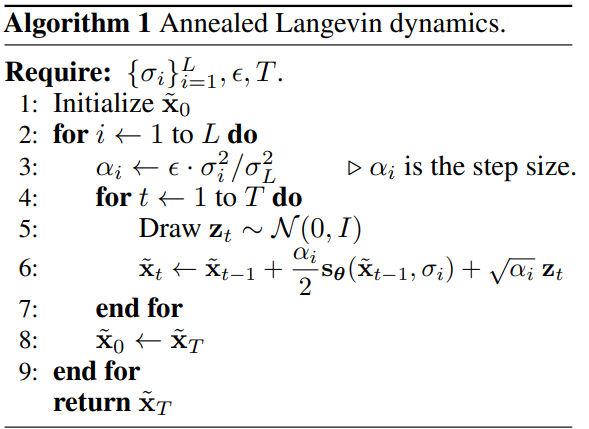
\includegraphics[scale=0.8]{算法1.png}
	\end{figure}

	我们先从均匀分布中采样$\bar{x}_0$,$s_{\theta}(x,1)$估计$\nabla_{\grave{x}} \log p_{\sigma_1}(\grave{x}|x)$,由于$\sigma_{1}$是一个较大的值,$s_{\theta}(x,1)$对$\nabla_{\grave{x}} \log p_{\sigma_1}(\grave{x}|x)$ 在低密度的区域估计也是准的,经过算法中的第二个for循环,我们最终关于$p_{\sigma_{1}}(\grave{x}|x)$的样本$x_T$是可以认为是关于对于分布$p_{\sigma_{1}}(\grave{x}|x)$的采样。
	
	显然$p_{\sigma_1}(\grave{x}|x)$与$p_{\sigma_2}(\grave{x}|x)$尽管略有不同,但是总体差别不大,经过利用$s_{\theta}(x,1)$迭代的样本$x_T$为$s_{\theta}(x,2)$提供了良好的初始化样本,也是就利用$s_{\theta}(x,2)$迭代的初始样本$x_0$是在$p_{\sigma_2}(\grave{x}|x)$的高密度区域,在高密度区域$s_{\theta}(x,2)$对$\nabla_{\grave{x}} \log p_{\sigma_2}(\grave{x}|x)$的估计是准的,以此类推,经过$s_{\theta}(x,i-1)$迭代优化的样本为$s_{\theta}(x,i)$提供了良好的初始化样本。
	
	最终$s_{\theta}(x,L-1)$迭代优化的样本为$s_{\theta}(x,L)$提供了高密度区域(密度梯度准确区域)采样的初始化样本,并且由于$\sigma_{L}$较小,$s_{\theta}(x,L)$可以看做是对$\nabla_{x} \log p_{data}(x)$的准确估计,进过迭代优化后得到了对$p_{data}(x)$的近似采样。
	
	关于$s_{\theta}(x,i)\quad i=1,...,L$,通常是使用U-NET结构,但是条件信息$i$如何输入网络中呢?DDPM使用NLP中的时间编码信息来表示而外的信息,这里使用条件实例归一化来表示。
	
	\subsubsection{\large{实例归一化:}}
	
	我们定义输入特征图$x$的形状为$(C,H,W)$,那么实例归一化首先对每个通道计算沿着空间维度的均值$\mu \in R^C$以及标准差$\varPhi \in R^C$:
	$$
		u_c=\dfrac{1}{HW}\sum_{h=1}^{H} \sum_{w=1}^{W} x_{\left[c,h,w\right]} \quad \quad  \varPhi_c =\sqrt{ \dfrac{1}{HW}\sum_{h=1}^{H} \sum_{w=1}^{W} \left( x_{\left[c,h,w\right]}-u_c \right)^2}   \quad \quad c=1,2,...,C
	$$
	
	我们设实例归一化的输出为$y$,形状为$(C,H,W)$,那么:
	$$
		y_{\left[ c,h,w \right]} = \gamma_{c} \dfrac{ x_{\left[ c,h,w \right]} - u_c }{\varPhi_c} + \beta_{c}
	$$
	其中$\gamma,\varPhi \in R^C$,是一组可学习的参数(线性映射系数)。
	
		
	\subsubsection{\large{条件实例归一化:}}
	
	与实例归一化不同的是,对于不同$i=1,...,L$使用不同的线性映射系数,我们重新定义$\gamma,\varPhi \in R^{  L \times C  }$,输出可以写成:
	$$
		y_{\left[ c,h,w \right]} = \gamma_{\left[ i,c \right]} \dfrac{ x_{\left[ c,h,w \right]} - u_c }{\varPhi_c} + \beta_{\left[  i,c \right]} \quad\quad \textbf{其中} i\text{为输入的条件}
	$$
	
	论文还做了一些修改:
	$$
		y_{\left[ c,h,w \right]} = \gamma_{\left[ i,c \right]} \dfrac{ x_{\left[ c,h,w \right]} - u_c }{\varPhi_c} + \beta_{\left[  i,c \right]} +\alpha_{\left[i,c\right]}\dfrac{u_c - m}{v} \quad\quad \textbf{其中} i\text{为输入的条件}
	$$
	
	式中$\alpha \in R^{L\times C}$是一组可以学习的参数,$m,v$分别为$u$的均值和标准差,我们把条件实例归一化放在所有的卷积层和池化层后面,对$s_{\theta}()$。
	\subsection{\Large SDE}
	
	
	
		
	
	
	
	
	
	
	
	
	
		
	
	

	
	
	
		
	

	
	
	

	
	

	
	
	
	
	
	
	
		
			
			


		
	
	
	
	
	
	
%	$x_{t+1}$的条件概率只依赖于$t$时刻的$x_t$,也就是:
%	$$
%	q(x_{t+1}|....,x_{t-1},x_{t})= q(x_{t+1}|x_t)
%	$$
	
	
	

		
		
		
		
		
		
	
	
	
	
	

  	
  	
  	
  	
 
 
 	
 	
 	
 	
	
	
	
	
	
	
	
\end{document}
	

